\documentclass{article}

\usepackage{listings}
\usepackage{color}
\usepackage{hyperref}
\usepackage{graphicx}
\usepackage{caption}
\usepackage{subcaption}



\title{Workflow on Running PHASTA}
\author{Fanlong Meng}
\begin{document}

\definecolor{mygreen}{rgb}{0,0.6,0}
\lstdefinestyle{myc}{
basicstyle=\footnotesize\ttfamily,
keywordstyle=\bfseries\color{mygreen}
}
\lstset{style=myc}

\maketitle

\section{Accounts}

In order to use PHASTA to solve fluid mechanics problems, you need to have access to either the SCOREC workstations or the CCI system.

You can contact Cameron Smith at 'smithc11 at rpi dot edu' to get access to the SCOREC computer. 

You can refer to the following FAQ webpage on how to get CCI account and access to CCI.


\url{https://secure.cci.rpi.edu/wiki/index.php/Frequently_Asked_Questions}

\section{Getting Started at SCOREC/CCI}

This chapter introduces new users to getting an environment set up on SCOREC and IBM BlueGene/Q workstation. It covers the most basic Linux configurations needed to compile the software stack and begin development.

\subsection{Connecting to the workstations}
\subsubsection{SCOREC}
After getting an account on SCOREC systems you should have a username and password. To access SCOREC systems, you must first go through the gateway machine at SCOREC called jumpgate. Running this from a terminal on your home computer will access jumpgate.
\begin{lstlisting}
  ssh myusername@jumpgate.scorec.rpi.edu
\end{lstlisting}
Enter your password at the prompt and you should end up logged into jumpgate. From here you can log in to any other SCOREC workstation. A list of workstations and their specs can be found here:\\
\url{https://www.scorec.rpi.edu/wiki/List_of_Computers}

Since you're already inside SCOREC systems, you don't need to repeat your username or scorec.rpi.edu.

\begin{lstlisting}
  ssh othello
\end{lstlisting}

\subsubsection{CCI}
The instructions of connecting to IBM BlueGene/Q workstation can be found in here: \\
\url{https://secure.cci.rpi.edu/wiki/index.php/Landing_Pad}

\subsection{File Systems}
\subsubsection{SCOREC}
There are several directories at SCOREC where you can put your files. The two most important ones are your home directory and your fast tmp directory. Your home directory is a safe place for important but not too large files. After logging in to a SCOREC machine your are in your home directory.
\begin{lstlisting}
  /users/myusername/
\end{lstlisting}
The /lore directory is a much bigger space suitable for keeping a copy of the SCOREC code for compiling and testing, as well as input and output data for your programs. However, any important code changes should be committed to the source code repository and important files should be moved to your home directory if possible. Here is the command to move to your /lore directory.
\begin{lstlisting}
  cd /lore/myusername/
\end{lstlisting}

These directories are conveniently available on all SCOREC machines, so they look the same no matter where you log in and changes made on one machine show up in another.

\subsubsection{CCI}
Basics about file system in CCI can be found in: \\
\url{https://secure.cci.rpi.edu/wiki/index.php/File\_System}

\subsection{Moving Files}

To move files to and from the SCOREC/CCI systems, a program similar to ssh called scp is useful. For example, to copy a file called mydata.txt from your home computer to your SCOREC/CCI home directory, run these on your home computer respectively.
\begin{lstlisting}
  scp mydata.txt myusername@jumpgate.scorec.rpi.edu:mydata.txt
\end{lstlisting}
\begin{lstlisting}  
  scp mydata.txt myusername@lp01.ccni.rpi.edu:mydata.txt
\end{lstlisting}

Similarly, to copy the same file from your SCOREC/CCI home directory onto your home computer, run these on your home computer respectively.

\begin{lstlisting}
  scp  myusername@jumpgate.scorec.rpi.edu:mydata.txt ./
\end{lstlisting}
\begin{lstlisting}  
  scp  myusername@lp01.ccni.rpi.edu:mydata.txt ./
\end{lstlisting}  
As you can see, scp is a lot like cp except the source and destination files can be on different machines.

\subsection{Compiling the Stack}

There are several pieces of third-party software required to compile SCOREC/CCI code, as well as other programs that you may find useful in development. For various reasons these are not available by default, and need to be activated through the module system. 

You can download the core tools 'core-sim'�� at:

\begin{lstlisting}
  cd
  cp -r /users/mengf5/coresim.tar.gz ./
  tar xzf coresim.tar.gz
\end{lstlisting}
for SCOREC workstations, and 
\begin{lstlisting}
  cd /gpfs/u/barn/myprojectname/myusername/
  cp -r /users/mengf5/coresimBGQ.tar.gz ./
  tar xzf coresimBGQ.tar.gz
\end{lstlisting}
for IBM BlueGene/Q workstation.

Then you have a new directory called 'core-sim' containing the code. Move into it.
\begin{lstlisting}
  cd core-sim
\end{lstlisting}

We have prepared a basic set of modules necessary to compile the code. This script should be executed once right after logging in to a workstation. For SCOREC you should run:
\begin{lstlisting}
source env-scorec.sh
\end{lstlisting}
The script for loading software dependencies on SCOREC systems env-scorec.sh won't work on IBM BlueGene/Q workstation. For IBM BlueGene/Q workstation you should run:
\begin{lstlisting}
source env-amos.sh
\end{lstlisting}

Now to compile the code for the first time. In the core directory, make a build directory to contain the compiled files and move into it
\begin{lstlisting} 
mkdir build
cd build
\end{lstlisting}

Next you will need to configure some options related to how the code is compiled. There is already an example script setting default options:
Compilation options are set by running CMake via the following script:
\begin{lstlisting}
source ../config.sh
\end{lstlisting}
where CMake is an extensible, open-source system that manages the build process, more info about CMake can be found in:\\
\url{http://www.cmake.org/overview/}

Now compiling all the code is as simple as running the following command.
\begin{lstlisting}
  make -j 4
  \end{lstlisting}

The -j 4 option tells the compilation system to compile 4 files at a time, which makes things faster on machines that have multiple cores.
Again, if all goes well you will not see any compilation errors.

\section{Build Pre-processor/Some Useful Tools/ and PHASTA Flow Solver}

\subsection{Build PHASTA pre-processor and Some Useful Tools}

After compelling the stack, build the PHASTA pre-processor 'chef:
\begin{lstlisting}
  make chef
\end{lstlisting}

then build the mesh format converter:
\begin{lstlisting}
make convert 
\end{lstlisting}

Meanwhile, you need to build the cadtosim to convert the model file from Parasolid format to Simmetrix format:
\begin{lstlisting}
cd core-sim/test/cadToSim/ 
./build.sh 
\end{lstlisting}

\subsection{Build PHASTA Flow Solver}

PHASTA is short for Parrallel Hierarchic Adaptive Stablized Transient Analysis.  PHASTA solver currently can model compressible or incompressible, laminar or turbulent, steady or unsteady flows in 3D, using unstructured grids. More reference about PHASTA can be found at:\\
\url{https://www.scorec.rpi.edu/wiki/PHASTA_Documentation} 

You can download the PHASTA code for SCOREC workstation following:
\begin{lstlisting}
  cd 
  cp -r /lore/cwsmith/develop/phasta.tar.gz ./
  tar xzf phasta.tar.gz
   \end{lstlisting}
for IBM BlueGene/Q workstation:
\begin{lstlisting}
  cd /gpfs/u/barn/myprojectname/myusername/
  cp -r /users/mengf5/phastaBGQ.tar.gz ./
  tar xzf phastaBGQ.tar.gz
   \end{lstlisting}
 
You need to clear the modules loaded for core-sim before building the PHASTA flow solver, then you can build the PHASTA flow solver following:
\begin{lstlisting}
  cd phasta
  source setEnv.sh
  cd mrPhasta
  mkdir build
  cd build
  ../../doConfigureGccMpich
  make
\end{lstlisting}


\section{Test case setup}

After compiling all the tools and programs, we can follow a test case demonstration to see how to solve fluid problem using PHASTA. 

The test case shown in Figure 1. is a crossflow problem. It represents an incompressible flow problem, and is solved by detached eddy simulation(DES). The governing equations are incompressible Navier-stokes(NS) equations and a transport equation for a turbulent viscosity. 
\begin{figure}[h!]
  \centering
    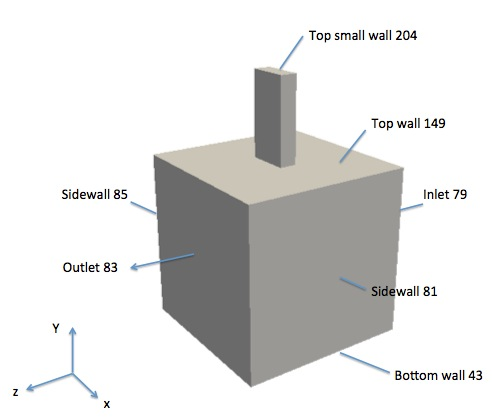
\includegraphics[width=0.7\textwidth]{fig1}
  \caption{Test case problem}
\end{figure}
The boundary conditions are:\\
At surface inlet 79, the inflow velocity is $v = v_z= 1$, the inflow turbulent viscosity is 5.4e-05.\\
At surface outlet 83, the outflow traction is 0, the outflow pressure is 0 and the derivative turbulent viscosity is 0. \\
At the top small wall 204, the turbulent viscosity is 0, and a sinusoidal in time jet velocity is given in y direction. \\
The top wall 149 and the four side walls of the top region(not labeled in Figure 1.) satisfies nonslip, non-penetration boundary condition, and the turbulent viscosity on the walls are equals to 0.\\
At side wall 81 and 85 in the big region, $v_x=0$, derivative of turbulent viscosity is 0 and the tractions on the wall are equals to 0.\\
At the bottom wall 43, $v_y=0$, derivative of turbulent viscosity is 0 and the tractions on the wall are equals to 0.\\
 
The initial condition for the problem is: \\
For the entire region, the initial velocity is $v = v_z = 1e-08$, the initial turbulent viscosity is 5.4e-05, the initial pressure is 0.0 \\ 

Except for solving incompressible NS equations, PHASTA is also able to solve Euler equations and compressible NS equations. Meanwhile, it can employ RANS, LES as well as DES as turbulent modeling. When it comes to multiphase flow, level-set method is also available in the program. Changing of solving strategies can be done by modifying solver.inp.

\section{Mesh Generation}

Before running PHASTA pre-processor 'chef', we need to generate a model file, a mesh file as well as an attribute file describing the problem boundary conditions and initial conditions.

The model file in Parasolid format with suffix .xmt\_txt can be used on SCOREC workstations. However, Since that the Parasolid modeling kernel is not available on the IBM BlueGene/Q, you have to use a model file in Simmetrix format with suffix .smd that is available. The mesh file will be used in 'chef' is required to be in SCOREC MDS format with suffix .smb.

First, we need to generate a Parasolid file(.xmt\_txt) using CAD software. To use this file on CCI, we can either convert it to smd file using following command:
  \begin{lstlisting}
  cadtosim <parasolid model> 
  \end{lstlisting}
which will create a new .smd model in your directory called translatedmodel.smd.

Then, we can generate the Simmetrix mesh file using Simmetrix SimModeler GUI. A detailed mesh generation tutorial can also be found in here:\\
\url{https://www.scorec.rpi.edu/researchwiki/SimModeler}.

The mesh file for the test case problem is shown in Figure 2. It is obvious that the mesh size is relatively small near the section with small section area since velocity change in that section is larger in this case. Also a 3D boundary layer is used in mesh generation on the highlighted surface. 
\begin{figure}[h!]
  \centering
    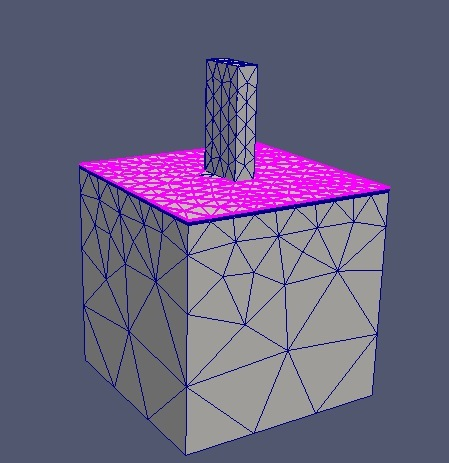
\includegraphics[width=0.7\textwidth]{fig2}
  \caption{Mesh of test case}
\end{figure}

After successfully generating the Simmetrix mesh (.sms file), there is a converter from the Simmetrix mesh format to the SCOREC mesh format.convert the Simmetrix mesh that you create into a Scorec mesh:
  \begin{lstlisting}
  convert <simmetrix model> <simmetrix mesh> <scorec mesh>
  \end{lstlisting}

With Simmetrix model and SCOREC mesh, you can generate the .spj file that specifies the boundary and initial conditions. The ascii text file for boundary conditions is the only supported way to define boundary/initial conditions for this version of 'chef', and can only be generated manually. More details about how to create the boundary/initial conditions in spj file can be found in the Chapter Boundary Conditions. 

You can download the test case for SCOREC workstation at:
   \begin{lstlisting}
  cd
  cp -r /users/mengf5/crossflow.tar.gz ./
  tar xzf crossflow.tar.gz
  \end{lstlisting}
for IBM BlueGene/Q workstation at:
  \begin{lstlisting}
  cd /gpfs/u/scratch/myprojectname/myusername/
  cp -r /users/mengf5/crossflowBGQ.tar.gz ./
  tar xzf crossflowBGQ.tar.gz
  \end{lstlisting}
In the crossflow folder, the you can find the mesh, model file in correct format and .spj file under /crossflow.

Other than generating a simple mesh like this case, SimModeler is able to generate a much more complex mesh. For example, figure 3 show a parallel unstructured mesh generation of 13 million element mesh on a complex geometric model from mesh controls defined in GUI. Figure 4 shows 16 parts of the 128 part partitioning of the 13 million element mesh of upright model.

\begin{figure}[h!]
  \centering
    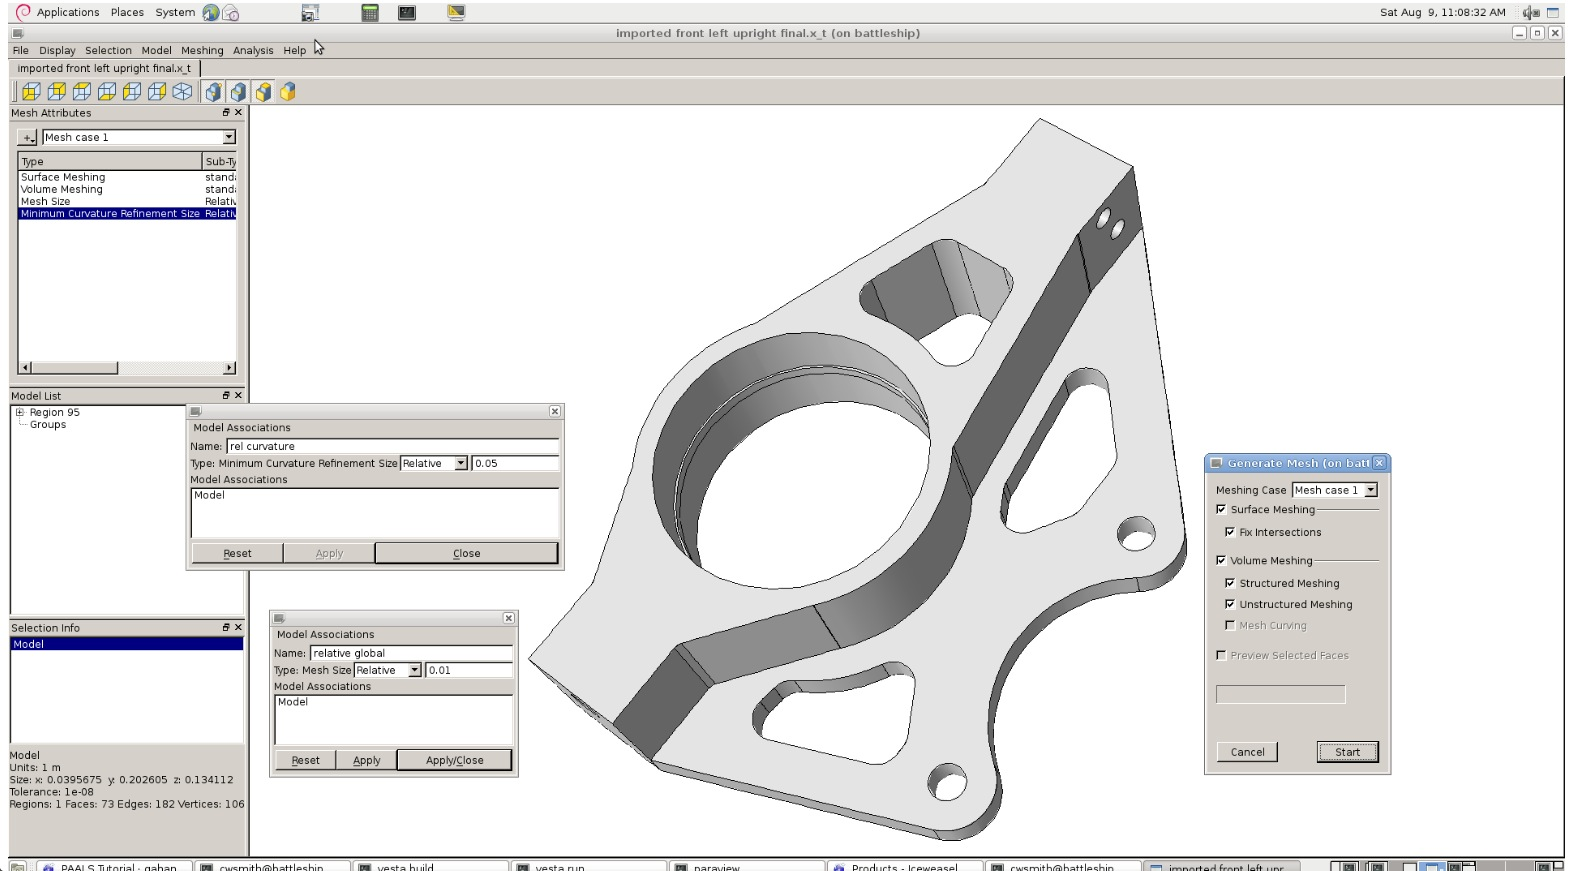
\includegraphics[width=0.7\textwidth]{albany1}
  \caption{Suspension upright from the RPI Formula Hybrid race car in SimModeler GUI}
\end{figure}
\begin{figure}[h!]
  \centering
    \includegraphics[width=0.7\textwidth]{albany2}
  \caption{Parts 0-15 of the 128 part partitioning of 13 million element mesh of upright model.}
\end{figure}

\pagebreak

\section{Boundary Conditions}

The boundary and initial conditions need to be specified in .spj file manually. In this Chapter, full names and abbreviations for boundary conditions as well as some comments are documented:
In .spj file, Essential boundary conditions are :
  \begin{lstlisting}
   density         D   rho
   temperature     T
   pressure        P
   comp1           C1
   comp3           C3
   scalar_1        S1  sc1
   scalar_2        S2  sc1
   scalar_3        S3  sc1
   scalar_4        S4  sc1
  \end{lstlisting}
,natural boundary conditions are:
  \begin{lstlisting}
   mass flux        MF
   natural pressure NP
   traction vector  TV
   heat flux        HF
 * turbulence wall  TW
   scalar_1 flux    F1
   scalar_2 flux    F2
   scalar_3 flux    F3
   scalar_4 flux    F4
 * surf ID          SID
  \end{lstlisting}
   Initial conditions are:
  \begin{lstlisting}
   initial pressure
   initial velocity
   initial temperature
   initial scalar_1
   initial scalar_2
   initial scalar_3
   initial scalar_4
  \end{lstlisting}
   A .spj file is composed of two kinds of lines, one is \# comments begin with a pound sign, and it is followed by a line describing: condition\_name: model\_id model\_dim c0 c1 c2 c3. \\
   The model\_id and model\_dim specify a geometric model entity. Typically model\_dim=2 for boundary conditions on model faces, or model\_dim=3 for initial conditions on model regions.\\
   All conditions have one component except for the following:\\
   comp1            4 \\
   comp3            4 \\
   initial velocity 3 \\
   traction vector  3 \\
   Both of comp1 and comp3 are essential boundary conditions affecting velocity. \\
   comp3 is a strict constraint, velocity = m*(x,y,z) \\
   comp1 is a planar constraint, dot(velocity,(x,y,z)) = m; \\
   Both are listed in the spj file as: m x y z \\
   Inital velocity and traction vector are both listed as: x y z
   The scalars 1 through 4 are not always present. \\
Note, Surf ID is an attribute which allows us to tag some faces. This is use to tell PHASTA to compute the force that applies on some tagged faces.
To apply a varying BC (both in time and space), in the test case problem the sinusoidal velocity on surface 204, we first set up a constant zero velocity profile in the .spj file (search for face 204 in geom.spj file). Then, with the additional Surf ID associated with this face, PHASTA can retrieve the vertices located on this face through the Surf ID attribute and prescribe a new velocity profile, which acts similarly to a new inlet. This prescribed velocity profile is implemented in phSolver/incompressible/BCprofie.f.

\section{Pre-processing}
After generating the required mesh files, you can run preprocessor 'chef' to partition the mesh and generate the PHASTA input files, for SCOREC workstation:
  \begin{lstlisting}
  cd crossflow
  source /users/myusername/core-sim/env-scorec.sh
  cd 4-1chef
  /users/myusername/coreSim/build/test/chef 
  \end{lstlisting}
For IBM BlueGene/Q workstation:
  \begin{lstlisting}
  cd crossflow
  module clear
  source /gpfs/u/barn/myprojectname/myusername/core-sim/env-amos.sh
  cd 4-1chef
  srun -t 5 -n 1 -o log /gpfs/u/barn/myprojectname/myusername/core-sim/build/test/chef
  \end{lstlisting}

This should create a 4-procs\_case directory containing the PHASTA input files in the posix format.

\section{Run PHASTA}

First run program converterO2N to generate PHASTA input files in the syncoIO format, then run PHASTA. For SCOREC workstations: 
  \begin{lstlisting}
  cd 4posixToSync
  mpirun -np 4 /path/to/phasta/mrPhasta/build/bin/converterO2N 
  cd 4solve
  mpirun -np 4 /path/to/phasta/mrPhasta/build/bin/phastaIC.exe 
  \end{lstlisting}
For IBM BlueGene/Q workstation:
  \begin{lstlisting}
  cd 4posixToSync
  srun -t 20 -n 4 -o log /gpfs/u/barn/myprojectname/myusername/phasta/ &  
  mrPhasta/build/bin/converterO2N
  cd 4solve
  srun -t 20 -n 4 -o log /gpfs/u/barn/myprojectname/myusername/phasta/ &
  mrPhasta/build/bin/phastaIC.exe
  \end{lstlisting}
Running coverterO2N should create a 4-procs\_case-SyncIO-1 directory containing phasta input files in the 'syncoIO' format.
Running PHASTA should create a 4-procs\_case directory containing restart-dat.[4|8|12|16|20].1 files in the posix format.

\section{Output}

One way to confirm that your solution is plausible is to compare the log file generated after running PHASTA with the reference file phasta\_4.log\_ref.

The following is a sample output from phSolver for one time step, due to the limited page size, the first four columns of output are displayed in the top table and the last four columns are displayed in the bottom one:
\begin{center}
    \begin{tabular}{| l | l | l | l |}
    \hline
    Timestep & CPU Time & Residual* & Normalized residual \\ \hline
    10 & 3.113E+02 & 1.676E-05 & (-10) \\ 
\hline
    \end{tabular}
\end{center}

\begin{center}
    \begin{tabular}{| l | l | l | l |}
\hline
Max(DeltaU/U) & Max(Deltap/P) & NOT RELEVANT& CG - GMRES iterations\\ \hline
      2.205E-02 & 3.361E-01 & 1215 -3 12  & [35-10] \\
    \hline
    \end{tabular}
\end{center}

*Where Residual is only the residual from the momentum and continuity equations.

The difference between residuals of your calculation and the reference should be very small. The small discrepancy is due to the partitioning generated by Chef is slightly different from the reference. Partitioning is indeed non deterministic so this should be fine. You can claim your run was successful if the difference here is small enough.

\section{Post-processing}

To visualize the results, you need to convert them from 'syncIO' format to 'posix' format. After running PHASTA, the output files(in posix format) can be visualized by using Paraview. Before running Paraview, you first need to convert the restart files to 'posix' format which is a readable format in Paraview. You can either use Paraview in SCOREC workstation or download it onto your own desktop through:
\url{www.paraview.org}

create 'IO.N2O.input' with the following content in folder /path/to/4solve:
   \begin{lstlisting}
  N-geombc-fields-double: 3;
  N-geombc-fields-integer: 20;
  N-restart-fields-double: 1;
  N-restart-fields-integer: 1;
  N-steps: 20;
  N-parts: 4;
  N-files: 1;
  restart, solution, double, block, 3;
  restart, ybar, double, block, 3;
  restart, errors, double, block, 3;
  restart, dwal, double, block, 3;
    \end{lstlisting}

where, N-steps is the total number of time-steps to load; N-parts is the total number of partitions/parts to load(the number of cores used for the calculation by PHASTA in this case 4)

then run converterN2O:
  \begin{lstlisting}
  mpirun -np 4 /path/to/phasta/mrPhasta/build/bin/converterN2O \&> log
  cat log
    \end{lstlisting}

This should create a 4-procs\_case-1PPP directory containing PHASTA output files in the 'posix' format.

Take geombc files in 'posix' format from the PHASTA input files to the new directory 4-procs\_case-1PPP:

  \begin{lstlisting}
  cd 4-procs\_case-1PPP
  cp ../../../4-1chef/4-procs-case/geombc.dat.* ./
    \end{lstlisting}

Now you have a full set of geombc and restart files in 'posix' format. Copy the phasta.pht file from the crossflow directory to the /4-procs\_case-1PPP directory. Open the phasta.pht file with Paraview to visualize the posix formatted PHASTA files.

Figure 5. shows a surface cutted at half plane in x-normal direction of turbulent viscosity. Figure 6. shows a contour plot of pressure filed.

\begin{figure}[h!]
  \centering
    \includegraphics[width=1\textwidth]{res1}
  \caption{A cut surface of turbulent viscosity}
\end{figure}

\begin{figure}[h!]
  \centering
    \includegraphics[width=1\textwidth]{res2}
  \caption{A contour of pressure field}
\end{figure}

\pagebreak


\end{document}
